\ifdefined\activerhandout 
\documentclass[12pt,aspectratio=1610,handout]{beamer}
\else
\documentclass[12pt,aspectratio=1610]{beamer}
\fi

%\usepackage[french]{babel} %=> erreur avec les tikz du moteur
\usepackage[T1]{fontenc}
\usepackage[utf8]{inputenc}
\usepackage{lmodern}
\usepackage{hyperref}
\usepackage{smartdiagram}
\usepackage{tikz}
\usepackage{animate}
\usepackage{tikzpeople}
\usepackage{appendixnumberbeamer}
\usepackage[labelformat=empty]{caption}
%\usepackage{pictochrono}
\usepackage{fontawesome5}
\usepackage{awesomebox}

\usetheme{Warsaw}
\setbeamertemplate{page number in head/foot}[totalframenumber]

\newcommand{\anglais}[1]{(\textit{\color{blue}#1})}
\newcommand{\legende}[2]{\caption[#1 (Source : \cite{#2})]{#1}}
\newcommand{\histoire}[1]{\begin{awesomeblock}{2pt}{\faBook}{black!75}#1\end{awesomeblock}}
\newcommand{\info}[1]{\begin{awesomeblock}{2pt}{\faInfoCircle}{black!75}#1\end{awesomeblock}}
\newcommand{\question}[1]{\begin{awesomeblock}{2pt}{\faQuestionCircle}{black!75}#1\end{awesomeblock}}
\newcommand{\alerte}[1]{\begin{awesomeblock}{2pt}{\faExclamationCircle}{black!75}#1\end{awesomeblock}}
\newcommand{\astuce}[1]{\begin{awesomeblock}{2pt}{\faLightbulb}{black!75}#1\end{awesomeblock}}
\newcommand{\exemple}[1]{\begin{awesomeblock}{2pt}{\faSearch}{black!75}#1\end{awesomeblock}}
\newcommand{\definitionAConnaitre}[1]{\begin{awesomeblock}{2pt}{\faCog}{black!75}#1\end{awesomeblock}}

\newcommand{\qmcBia}[7]{
%1 : titre slide
%2 : numéro de la bonne réponse
%3 : Inititulé de la question
%4, 5, 6, et 7 : propositions de réponse
\begin{frame}{#1}
\begin{awesomeblock}{2pt}{\faQuestion}{black!75}
#3
	\begin{enumerate}
	\ifnum#2=1
		\only<1>{\item #4}
		\only<2>{\item \textbf{#4}}
	\else
		\item #4
	\fi
	\ifnum#2=2
		\only<1>{\item #5}
		\only<2>{\item \textbf{#5}}
	\else
		\item #5
	\fi
	\ifnum#2=3
		\only<1>{\item #6}
		\only<2>{\item \textbf{#6}}
	\else
		\item #6
	\fi
	\ifnum#2=4
		\only<1>{\item #7}
		\only<2>{\item \textbf{#7}}
	\else
		\item #7
	\fi
	\end{enumerate}
	\pause
\end{awesomeblock}
\end{frame}
}

\subtitle{BIA - Brevet d'Initiation Aéronautique}
\author{Clément \textsc{Vermot-Desroches}}
\institute{Collège Aliénor d'Aquitaine\\Martignas-sur-Jalle}
\date{\today}

%\AtBeginSection[]
%{
%    \begin{frame}
%        %\frametitle{Table of Contents}
%        \tableofcontents[currentsection]
%    \end{frame}
%}

\AtBeginSubsection[]
{
    \begin{frame}
        %\frametitle{Table of Contents}
        \tableofcontents[currentsection,currentsubsection]
    \end{frame}
}
%éléments communalisés
\pgfdeclareimage{case}{01-EtudeAeronefs/img/instruments/alt/alt_case.pdf}

\pgfdeclareimage{asiFace}{01-EtudeAeronefs/img/instruments/asi/asi_face.pdf}
\pgfdeclareimage{asiHand}{01-EtudeAeronefs/img/instruments/asi/asi_hand.pdf}
\pgfdeclareimage{asiCase}{01-EtudeAeronefs/img/instruments/asi/asi_case.pdf}

\pgfdeclareimage{altCase}{01-EtudeAeronefs/img/instruments/alt/alt_case.pdf}
\pgfdeclareimage{altFace1}{01-EtudeAeronefs/img/instruments/alt/alt_face_1.pdf}
\pgfdeclareimage{altFace2}{01-EtudeAeronefs/img/instruments/alt/alt_face_2.pdf}
\pgfdeclareimage{altFace3}{01-EtudeAeronefs/img/instruments/alt/alt_face_3.pdf}
\pgfdeclareimage{altHand1}{01-EtudeAeronefs/img/instruments/alt/alt_hand_1.pdf}
\pgfdeclareimage{altHand2}{01-EtudeAeronefs/img/instruments/alt/alt_hand_2.pdf}

\pgfdeclareimage{aiCase}{01-EtudeAeronefs/img/instruments/ai/ai_case.pdf}
\pgfdeclareimage{aiFace}{01-EtudeAeronefs/img/instruments/ai/ai_face.pdf}
\pgfdeclareimage{aiRing}{01-EtudeAeronefs/img/instruments/ai/ai_ring.pdf}
\pgfdeclareimage{aiBack}{01-EtudeAeronefs/img/instruments/ai/ai_back.pdf}

\pgfdeclareimage{hiCase}{01-EtudeAeronefs/img/instruments/hi/hi_case.pdf}
\pgfdeclareimage{hiFace}{01-EtudeAeronefs/img/instruments/hi/hi_face.pdf}

\pgfdeclareimage{tcCase}{01-EtudeAeronefs/img/instruments/tc/tc_case.pdf}
\pgfdeclareimage{tcFace1}{01-EtudeAeronefs/img/instruments/tc/tc_face_1.pdf}
\pgfdeclareimage{tcFace2}{01-EtudeAeronefs/img/instruments/tc/tc_face_2.pdf}
\pgfdeclareimage{tcBall}{01-EtudeAeronefs/img/instruments/tc/tc_ball.pdf}
\pgfdeclareimage{tcBack}{01-EtudeAeronefs/img/instruments/tc/tc_back.pdf}
\pgfdeclareimage{tcMark}{01-EtudeAeronefs/img/instruments/tc/tc_mark.pdf}

\pgfdeclareimage{vsiCase}{01-EtudeAeronefs/img/instruments/vsi/vsi_case.pdf}
\pgfdeclareimage{vsiHand}{01-EtudeAeronefs/img/instruments/vsi/vsi_hand.pdf}
\pgfdeclareimage{vsiFace}{01-EtudeAeronefs/img/instruments/vsi/vsi_face.pdf}

\pgfdeclareimage{ilsCase}{01-EtudeAeronefs/img/instruments/ils/ils_case.pdf}
\pgfdeclareimage{ilsCaseFixed}{01-EtudeAeronefs/img/instruments/ils/ils_case_fixed.pdf}
\pgfdeclareimage{ilsFace}{01-EtudeAeronefs/img/instruments/ils/ils_face.pdf}
\pgfdeclareimage{ilsFlagGs}{01-EtudeAeronefs/img/instruments/ils/ils_flag_gs.pdf}
\pgfdeclareimage{ilsFlagNav}{01-EtudeAeronefs/img/instruments/ils/ils_flag_nav.pdf}
\pgfdeclareimage{ilsHandGs}{01-EtudeAeronefs/img/instruments/ils/ils_hand_gs.pdf}
\pgfdeclareimage{ilsHanvNav}{01-EtudeAeronefs/img/instruments/ils/ils_hand_nav.pdf}

%altimètre
%   -paramètre 1 : altitude en pieds
%   -paramètre 2 : calage en pouces de mercure
\def\alti#1#2{
	\fill[transparent] (0,0) circle (3) ;
	\node[rotate=(#2-28.0)*100] {\pgfbox[center,center]{\pgfuseimage{altFace1}}};
	\node {\pgfbox[center,center]{\pgfuseimage{altFace2}}};
  	\node[rotate=-{(Mod(#1/10,10000))*(36/1000)}] {\pgfbox[center,center]{\pgfuseimage{altFace3}}};
  	\node[rotate=-{(Mod(#1,1000))*(360/1000)}] {\pgfbox[center,center]{\pgfuseimage{altHand2}}};
    	\node[rotate=-{(Mod(#1,10000))*(360/10000)}] {\pgfbox[center,center]{\pgfuseimage{altHand1}}};
    	%\node {\pgfbox[center,center]{\pgfuseimage{altCase}}};
	\node {\pgfbox[center,center]{\pgfuseimage{case}}};
}

%consevateur de cap
%   -paramètre 1 : cap en degrés
\def\conservateurCap#1{
	\fill[transparent] (0,0) circle (3) ;
  	\node[rotate=#1] {\pgfbox[center,center]{\pgfuseimage{hiFace}}};
    	\node {\pgfbox[center,center]{\pgfuseimage{hiCase}}};
}

%ILS
%   -paramètre 1 : QDM en degrés
%   -paramètre 2 : décallage horizontal
%   -paramètre 3 : décallage vertical
\pgfkeys{
    /ilsparam/.is family,
    /ilsparam,
    qdm/.store in = \ilsQdm,
    ecartLoc/.store in = \ilsEcartLoc,
    ecartGlide/.store in = \ilsEcartGlide,
    afficherFlagNav/.store in = \ilsAfficherFlagNav,
    afficherFlagGs/.store in = \ilsAfficherFlagGs,
    qdm = 0,
    ecartLoc = 0,
    ecartGlide = 0,
    afficherFlagNav = false,
    afficherFlagGs = false,
}
\newcommand{\ils}[1]{
    \pgfkeys{/ilsparam, #1}
%\def\ils#1#2#3{
	\fill[transparent] (0,0) circle (3) ;
		\node {\pgfbox[center,center]{\pgfuseimage{ilsCaseFixed}}};
		\ifthenelse{\equal{\ilsAfficherFlagGs}{true}}{
			\node {\pgfbox[center,center]{\pgfuseimage{ilsFlagGs}}};
		}
		\ifthenelse{\equal{\ilsAfficherFlagNav}{true}}{
			\node {\pgfbox[center,center]{\pgfuseimage{ilsFlagNav}}};
		}
		\node[yshift=\ilsEcartGlide*31.75] {\pgfbox[center,center]{\pgfuseimage{ilsHandGs}}};
		\node[xshift=\ilsEcartLoc*31.75] {\pgfbox[center,center]{\pgfuseimage{ilsHanvNav}}};
		\node[rotate=\ilsQdm] {\pgfbox[center,center]{\pgfuseimage{ilsFace}}};
    	\node {\pgfbox[center,center]{\pgfuseimage{ilsCase}}};
}

%variomètre
%   -paramètre 1 : taux de descente
\def\vario#1{
	\fill[transparent] (0,0) circle (3) ;
  	\node {\pgfbox[center,center]{\pgfuseimage{vsiFace}}};
   	\node[rotate=-(#1/2000)*172] {\pgfbox[center,center]{\pgfuseimage{vsiHand}}};
    	%\node {\pgfbox[center,center]{\pgfuseimage{vsiCase}}};
	\node {\pgfbox[center,center]{\pgfuseimage{case}}};
}

%horizon
%   -paramètre 1 : roulis
%   -parametre 2 : tangage 
\def\horizon#1#2{
	\fill[transparent] (0,0) circle (3) ;
	\node {\pgfbox[center,center]{\pgfuseimage{aiBack}}};
  	\node[rotate=#1,yshift=-#2*1.25] {\pgfbox[center,center]{\pgfuseimage{aiFace}}};
    	\node[rotate=#1] {\pgfbox[center,center]{\pgfuseimage{aiRing}}};
    	\node {\pgfbox[center,center]{\pgfuseimage{aiCase}}};
}

%indicateur de virage
%   -paramètre 1 : taux virage [-1;1] 
%   -parametre 2 : postion bille [-1;1] 
\def\indicateurVirage#1#2{
	\fill[transparent] (0,0) circle (3) ;
  	\node {\pgfbox[center,center]{\pgfuseimage{tcBack}}};
    	\node {\pgfbox[center,center]{\pgfuseimage{tcFace1}}};
    	\node {\pgfbox[center,center]{\pgfuseimage{tcFace2}}};
    	%\node[xshift=#2*35,yshift=#2*4] {\pgfbox[center,center]{\pgfuseimage{tcBall}}};
	\node[rotate around={#2*15:(0,3.7)}] {\pgfbox[center,center]{\pgfuseimage{tcBall}}};
    	\node[rotate=#1*20] {\pgfbox[center,center]{\pgfuseimage{tcMark}}};
    	%\node {\pgfbox[center,center]{\pgfuseimage{tcCase}}};
	\node {\pgfbox[center,center]{\pgfuseimage{case}}};
}

%badin
%   -paramètre 1 : vitesse [0;200] 
\def\badin#1{
	\fill[transparent] (0,0) circle (3) ;
  	\node {\pgfbox[center,center]{\pgfuseimage{asiFace}}};
    	
	%0 kts : 0°
	%40 kts : 36°
	%70 kts : 90°
	%130 kts : 210°
	%160 kts : 264°
	%200 kts : 312°

	%	Vitesse	Position aiguille	Angle/10 kts
	%	0		0,00°	
	%	40		36,00°		NA
	%	50		54,00°		-18°
	%	60		72,00°		-18°
	%	70		90,00°		-18°
	%	80		110,00°		-20°
	%	90		130,00°		-20°
	%	100		150,00°		-20°
	%	110		170,00°		-20°
	%	120		190,00°		-20°
	%	130		210,00°		-20°
	%	140		228,00°		-18°
	%	150		246,00°		-18°
	%	160		264,00°		-18°
	%	200		312,00°		-12°

	%Entre 0 et 40 kts
	\ifnum#1<41
	\node[rotate=-(((#1)/(40))*(36))] {\pgfbox[center,center]{\pgfuseimage{asiHand}}};
	\fi 
	%Entre 40 et 70 kts
	\ifnum#1>40 \ifnum#1<71
	\node[rotate=-(((#1-40)/(70-40))*(90-36))-36] {\pgfbox[center,center]{\pgfuseimage{asiHand}}};
	\fi \fi
	%Entre 71 et 130 kts
	\ifnum#1>70 \ifnum#1<131
	\node[rotate=-(((#1-70)/(130-70))*(210-90))-90] {\pgfbox[center,center]{\pgfuseimage{asiHand}}};
	\fi \fi
	%Entre 130 et 160 kts
	\ifnum#1>130 \ifnum#1<161
	\node[rotate=-(((#1-130)/(160-130))*(264-210))-210] {\pgfbox[center,center]{\pgfuseimage{asiHand}}};
	\fi \fi
	%Entre 160 et 200 kts
	\ifnum#1>160
	\node[rotate=-(((#1-160)/(200-160))*(312-264))-264] {\pgfbox[center,center]{\pgfuseimage{asiHand}}};
	\fi

    	%\node {\pgfbox[center,center]{\pgfuseimage{asiCase}}};
	\node {\pgfbox[center,center]{\pgfuseimage{case}}};
}

% Définir les clés pour les paramètres
\pgfkeys{
    /tdb/.is family,
    /tdb,
    vitesse/.store in = \tdbVitesse,
    altitude/.store in = \tdbAltitude,
    calageAltitude/.store in = \tdbCalageAltitude,
    vz/.store in = \tdbVz,
    cap/.store in = \tdbCap,
    assiette/.store in = \tdbAssiette,
    inclinaison/.store in = \tdbInclinaison,
    derapage/.store in = \tdbDerapage,
    virage/.store in = \tdbVirage,
    afficherT/.store in = \tdbAfficherT,
    vitesse = 0,
    altitude = 0,
    vz = 0,
    cap = 0,
    assiette = 0,
    inclinaison = 0,
    derapage = 0,
    virage = 0,
    calageAltitude = 30,
    afficherT = false,
}

%Planche de bord
\newcommand{\dessinerTdB}[1]{
    \pgfkeys{/tdb, #1}

    \begin{tikzpicture}
        % Définir les coordonnées des sommets de la planche de bord
        \coordinate (A) at (-5, 3.5);
        \coordinate (B) at (19, 3.5);
        \coordinate (C) at (19, -10.5);
        \coordinate (D) at (-5, -10.5);

        % Dessiner le polygone avec le coin supérieur gauche arrondi
        \fill[gray, rounded corners=3cm] (D) -- (A) -- (B) -- (C) -- cycle ;

        % Dessiner le polygone rouge si showredpolygon est vrai
        \ifthenelse{\equal{\tdbAfficherT}{true}}{
            \coordinate (T1) at (-3.2, 3.2);
            \coordinate (T2) at (17.2, 3.2);
            \coordinate (T3) at (17.2, -3.5);  
            \coordinate (T4) at (10.4, -3.5);
            \coordinate (T5) at (10.4, -10.2);
            \coordinate (T6) at (3.6, -10.2);
            \coordinate (T7) at (3.6, -3.5); 	
            \coordinate (T8) at (-3.2, -3.5); 
            \draw[line width=5pt, red] (T1) -- (T2) -- (T3) -- (T4) -- (T5) -- (T6) -- (T7) -- (T8) -- cycle  ;
        }{}

        % Placer les instruments
        \begin{scope}[xshift=0cm, yshift=0cm]
            \badin{\tdbVitesse}
        \end{scope}
        
        \begin{scope}[xshift=7cm, yshift=0cm]
            \horizon{\tdbInclinaison}{\tdbAssiette}
        \end{scope}
        
        \begin{scope}[xshift=14cm, yshift=0cm]
            \alti{\tdbAltitude}{\tdbCalageAltitude}
        \end{scope}
        
        \begin{scope}[xshift=0cm, yshift=-7cm]
            \indicateurVirage{\tdbVirage}{\tdbDerapage}
        \end{scope}
        
        \begin{scope}[xshift=7cm, yshift=-7cm]
            \conservateurCap{\tdbCap}
        \end{scope}
        
        \begin{scope}[xshift=14cm, yshift=-7cm]
            \vario{\tdbVz}
        \end{scope}

        %\draw (B) grid (D);    
        
    \end{tikzpicture}
}


%\documentclass[tikz,border=6pt]{standalone}
%\usepackage{tikz}
\usetikzlibrary{calc,backgrounds}
%\usepackage{ifthen}

%\begin{document}

\pgfdeclareimage{montagne}{commun/img/montagne.pdf}

\newcommand{\echelleAltitudeMetres}[2]{
%\begin{tikzpicture}[x=1cm,y=1cm, scale=0.6, every node/.style={scale=0.6}] % 1 unité = 1 km = 1000 m

% --------- paramètres (modifiables) ----------
\def\maxkm{#1}            % hauteur totale en km (10 = 10000 m)
\def\pointeralt{#2}      % position curseur en km (5 = 5000 m)
\def\pointerside{right}   % 'left' ou 'right' (placement du curseur)
% limites horizontales de la montagne (choisis des valeurs <= -1.6 pour ne pas empiéter sur l'axe)
\def\positionMontagne{-4.9}      % bord gauche de la base
% ---------------------------------------------

% configuration curseur selon côté
\ifthenelse{\equal{\pointerside}{right}}{%
  \def\pointerx{0.45}%
  \def\labelanchor{west}%
  \def\xshift{6pt}%
}{%
  \def\pointerx{-0.45}%
  \def\labelanchor{east}%
  \def\xshift{-6pt}%
}

% cadre optionnel pour cadrer
	\draw[gray!0] (\positionMontagne,0) rectangle (2.5,\maxkm+0.3);

% Axe vertical (altitude)
\draw[line width=0.6pt] (0,0) -- (0,\maxkm+0.3);
% graduations 1000 m (1 km)
\foreach \k in {0,...,10}{
  \pgfmathtruncatemacro{\lab}{\k*1000}
  \draw (-0.12,\k) -- (0.12,\k);
  \node[left=3pt] at (-0.15,\k) {\small \lab\ m};
}
% étiquette d'axe "Altitude" déplacée plus à gauche pour ne pas être masquée
\node[rotate=90] at (-2.0,\maxkm/2) {\large Altitude};

\node at (\positionMontagne,0) {\pgfbox[0,0]{\pgfuseimage{montagne}}};

% --- Curseur triangulaire bleu sur le côté choisi (par défaut à droite) ---
\begin{scope}
  \fill[blue!70!black] (0,\pointeralt) -- (\pointerx,\pointeralt+0.22) -- (\pointerx,\pointeralt-0.22) -- cycle;
  \draw[blue!90!black,line width=0.6pt] (0,\pointeralt) -- (\pointerx,\pointeralt+0.22) -- (\pointerx,\pointeralt-0.22) -- cycle;
  \pgfmathtruncatemacro{\pointerm}{\pointeralt*1000}
  \node[anchor=\labelanchor, xshift=\xshift] at (\pointerx,\pointeralt) {\small \pointerm\ m};
\end{scope} 
}


%\end{tikzpicture}
%\end{document}


\title[Séance 6 - Instruments]{Séance 6 \\ Instruments de bord}

\begin{document}
 \begin{frame}
 \titlepage
 \end{frame}
 
 \begin{frame}
 \tableofcontents
 \end{frame}
 
 \section{Les instruments de bord}
	\begin{frame}{Instruments de bord, pourquoi ?}
	\question{Quelles informations sont nécessaires pour piloter un avion ?}
	\end{frame}	 
	
	\begin{frame}{Instruments de bord, pourquoi ?}
		\begin{figure}
			% [trim={left bottom right top},clip]
			\includegraphics[width=0.93\linewidth,trim={0 3cm 0 9cm},clip]{01-EtudeAeronefs/img/DR400plancheDeBord.jpg}
			\legende{Cockpit de DR400}{img:DR400plancheDeBord}
		\end{figure}	
	\end{frame}	 

 	\begin{frame}{Anémomètre}
 		\begin{columns}
 		\begin{column}{0.45\textwidth}
		\begin{figure}	
		\centering
			\begin{tikzpicture}
				\badin{110}
			\end{tikzpicture}
		\legende{Un "badin"}{tikz:instrumentsBase}
		\end{figure}
		\end{column}
 		\begin{column}{0.55\textwidth}
 			Indique la vitesse
 			
 			Les arcs représentent différentes vitesses :
 			\begin{itemize}
 				\item arc blanc : vitesse avec volets sortis (VFE, Velotcity Flaps Extended)
 				\item arc vert : vitesse en air turbulent (VNO, Velocity Normal Operating)
 				\item arc jaune : vitesse en air calme
 				\item trait rouge : vitesse à ne jamais dépasse (VNE, Velocty Never Exced)
 			\end{itemize}
 		\end{column}
 		\end{columns}
	\end{frame}	
	
	\begin{frame}{Anémomètre - fonctionnement}
		\begin{columns}
 		\begin{column}{0.58\textwidth}
		\begin{figure}
			% [trim={left bottom right top},clip]
			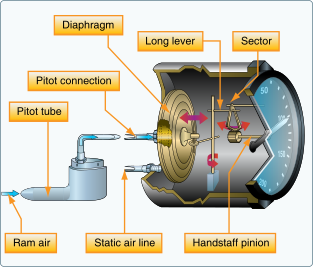
\includegraphics[width=1\linewidth]{01-EtudeAeronefs/img/instruments/schemaBadin.pdf}
			\legende{Fonctionnement d'un badin}{img:schemaBadin}
		\end{figure}	
		\end{column}
		\begin{column}{0.42\textwidth}
		\pause
		\histoire{L'anémomètre qui équipe nos avions a été inventé en 1911 par l'ingénieur français Raoul Badin, qui a donc donné son nom à cet instrument.}
		
		\histoire{Le tube Pitot a été inventé en 1732 par le physicien français Henri Pitot.}
		\end{column}
		\end{columns}
	\end{frame}	
	
	\begin{frame}{Anémomètre - mesure}
		\begin{figure}
			% [trim={left bottom right top},clip]
			\includegraphics[width=0.8\linewidth]{01-EtudeAeronefs/img/tubesPitotG6000}
			\legende{Pitot sur le fuselage d'un avion}{img:tubesPitotG6000}
		\end{figure}	
	\end{frame}
	\begin{frame}{Anémomètre - mesure}
		\begin{figure}
			% [trim={left bottom right top},clip]
			\includegraphics[width=0.8\linewidth]{01-EtudeAeronefs/img/tubePitotC172}
			\legende{Pitot sur un Cessna 172}{img:tubePitotC172}
		\end{figure}	
	\end{frame}
	
	
	\begin{frame}{Altimètre}
 		\begin{columns}
 		\begin{column}{0.45\textwidth}
		\begin{figure}	
		\centering
			\begin{tikzpicture}
				\altiHpa{4500}{1015}
			\end{tikzpicture}
		\legende{Un altimètre}{tikz:instrumentsBase}
		\end{figure}
		\end{column}
 		\begin{column}{0.55\textwidth}
 			Indique l'altitude
 			
 			Le "calage" de l'altimètre est modifiable pour permettre de prendre en compte la variabilité de la pression atmosphérique dans le temps et dans l'espace
 		\end{column}
 		\end{columns}
	\end{frame}
	
	\begin{frame}{Altimètre - réglage du calage}
 		\begin{columns}
 		\begin{column}{0.45\textwidth}
		\begin{figure}	
			\altiAnimReglageQnhHpa{360}{1500}{970}{1035}
			\legende{Effet du réglage du QNH}{img:schemaAltimetre}
		\end{figure}
		\end{column}
 		\begin{column}{0.55\textwidth}
 			
 		\end{column}
 		\end{columns}
	\end{frame}
	
	
 
\appendix 
\section{QCM}
\qmcBia{Météo}
{1}{Les deux principaux composants de l'air sec sont :}
{le diazote et le dioxygène}
{l'oxygène et le gaz carbonique}
{l'azote et l'hélium}
{l'oxygène et l'hydrogène} 
{}
 
\ifdefined\activerbibliobeamer
\begin{frame}[allowframebreaks]
\frametitle{Bibliographie}
\printbibliography
%\nocite{*}
\end{frame}
\fi 
 
\end{document}
